\section{Zyklische Graphen}
\begin{definition}
	\label{def:zyklus}
Ein \emph{einfacher Zyklus} oder ein \emph{einfacher Kreis} in einem Graphen $G=(V,E)$ ist ein einfacher Weg $\pi =v_0,\ldots,v_r$ mit $v_0=v_r$ und $r\ge2$ (im Falle von Digraphen) oder $r \ge 3$ (im Falle von ungerichteten Graphen).
Ein \emph{Zyklus} oder \emph{Kreis} ist ein Weg, ,der sich aus einfachen Zyklen zusammensetzt.
\end{definition}

\begin{remark}
Aus der Definition \ref{def:zyklus} folgt:
\begin{itemize}
	\item Jeder einfache Zyklus ist ein Zyklus
	\item Sind $\pi_1= v_0,\ldots, v_r$, $\pi_2=w_0,\ldots,w_s$ mit $v_i=w_0=w_r$ so ist auch \\ $\pi=v_0,\ldots,v_{i-1},w_0,\ldots,w_s,v_{i+1},\ldots, v_r$ ein Zyklus
	\item Es gibt keine andere Möglichkeit um Zyklen zu generieren.
\end{itemize}
\end{remark}
\begin{example}
Der Digraph 
\begin{center}
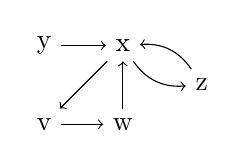
\begin{tikzpicture}
	\node (x) at (0,0) {x};
	\node (y) at (-1,0) {y};
	\node (v) at (-1,-1) {v};
	\node (w) at (0,-1) {w};
	\node (z) at (1,-0.5) {z};

	\path [->] (y) edge node {} (x);
	\path [->] (x) edge[bend right=30]  node {} (z);
	\path [->] (w) edge node {} (x);
	\path [->] (v) edge node {} (w);
	\path [->] (x) edge node {} (v);
	\path [->] (z) edge[bend right=30]  node {} (x);
\end{tikzpicture}
\end{center}
besitzt die einfachen Zyklen:
\begin{align*}
	\pi_1&=x,z,x \\
	\pi_2&=v,w,x,w
\end{align*}
und die nicht einfachen Zyklen:
\begin{align*}
	\pi_3&= x,z,x,z,x \\
	\pi_4&= v,w,x,z,x,v
\end{align*}
Der dazugehörige ungerichtete Graph:
\begin{center}
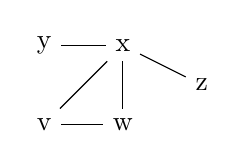
\begin{tikzpicture}
        \node (x) at (0,0) {x};
        \node (y) at (-1,0) {y};
        \node (v) at (-1,-1) {v};
        \node (w) at (0,-1) {w};
        \node (z) at (1,-0.5) {z};
        
        \path [-] (y) edge node {} (x);
        \path [-] (w) edge node {} (x);
        \path [-] (v) edge node {} (w);
        \path [-] (x) edge node {} (v);
        \path [-] (z) edge node {} (x);
\end{tikzpicture}
\end{center}
besitzt den einfachen Zyklus
\[
\pi_1= v,w,x,v
\]
Die Wege 
\begin{align*}
	\pi_2&= x,y,x \\
	\pi_3&=v,w,x,y,x,v
\end{align*}
sind keine Zyklen.
\end{example}
\subsection{Eulergraphen}
Im Folgenden betrachten wir exemplarisch das Königsberger Brückenproblem.
\begin{fluff}
Das Königsbergerbrückenproblem ist ein von Leonhard Euler gelöstes mathematisches Problem. Es handelt konkret um die Stadt Königsberg und um die Frage, ob es einen Rundweg gibt, bei dem man alle sieben Brücken der Stadt über den Pregel exakt einmal überqueren kann und wieder zum Ausgangspunkt gelangt.
\\ Euler zeigte, dass es keinen solchen Rundweg gibt.
\end{fluff}
\begin{definition}
Ein \emph{Eulerscher Rundweg} in einem Graphen $G=(V,E)$ ist ein Zyklus, der jede Kante $e \in  E$ genau einmal enthält. Im ungerichteten Fall nennen wir $G$ \emph{Eulersch}, falls der Grad jedes Knotens gerade ist. \\
Ein Digraph ist Eulersche, falls $indeg(v)= outdeg(v), v \in  V$.
\end{definition}
\begin{theorem}
	\label{thm:eulergraph}
	Ein zusammenhängender Graph $G=(V,E)$ besitzt genau dann einen Eulerschen Rundweg, falls der Graph Eulersch ist.
\end{theorem}
\begin{proof}
Hin- und Rückrichtung
\begin{itemize}
	\item \underline{$\implies$} Ein Knoten $v \in  V$ in einem Eulerschen Graph, der k-mal in einem Eulerschen Rundweg vorkommt, muss im gerichteten Fall
		\[
		indeg(v) =outdeg(v)
		\]
und im ungerichteten Fall
\[
deg(v)=2k
\]
erfüllen.
\item \underline{$\impliedby$} Sei $G$ Eulersch und $\pi=v_0,\ldots,v_r$ der längste Weg, in dem jede Kante aus $E$ höchstens einmal vorkommt.
Dies bedeutet, dass jede ausgehende Kante von $v_r$ im Weg enthalten sein muss (sonst wäre es nicht der längste Weg).
Die Bedingung an den Knotengrad impliziert: $v_0=v_r$.
\paragraph{Annahme:}
\begin{itemize}
	\item Digraphen: Es gibt eine Kante $e=(w_1,w_2) \in  E $ mit $e \neq (v_i, v_{i+1}, i=0,\ldots,r-1$
	\item ungerichtete Graphen: Es gibt eine Kante $e=\{w_1,w_2\} \in  E$ mit $e \neq \{v_i,v_{i+1}\}, i=0,\ldots,r-1$.
\end{itemize}
\underline{Fall 1:} $w_1 \text{ oder }w_2$ sind in $\pi$ enthalten. \\
Ohne Beschränkung der Allgemeinheit: $v_r=w_1$
\[
\implies \tilde{\pi} =v_0,\ldots,v_r,w_2
\]
Dies ist ein Widerspruch zur Annahme, da $\pi$ nun nicht mehr der längste Weg ist. \\
\underline{Fall 2:} $w_1$ und $w_2$ sind beide nicht in $\pi$ enthalten.
Da $G$ zusammenhängend ist, gibt es einen Weg von $v_0$ nach $w_1$. Entlang dieses Weges muss es eine Kante geben, die einen Knoten in $\pi$ und einen nicht in $\pi$ hat. \\
Analog zum ersten Fall führt dies zum Widerspruch.
\end{itemize}
\end{proof}
Wir beachten: Satz \ref{thm:eulergraph} ist die Antwort auf das Königsberger Brückenproblem. Demnach gibt es keinen solchen Weg und es ist nicht mögliche einen Euler-Weg zu finden.
